\ifx\FORMAT\undefined
\documentclass[11pt]{book}
\usepackage{amsmath,mathtools}
\usepackage[utf8]{inputenc}
\usepackage[ngerman]{babel}
\usepackage[T1]{fontenc}
\usepackage{lmodern}
\usepackage{acronym}
\usepackage{graphicx} 
\usepackage{epstopdf}
\usepackage{svg}
\usepackage{multirow}
\usepackage{amssymb}
\usepackage{trfsigns}
\usepackage{setspace}
\usepackage{yfonts}
\usepackage{nomencl}
\usepackage{float}
\usepackage{subfig}
\usepackage{scrpage2}
\usepackage{afterpage}
\usepackage{longtable}

\onehalfspacing


%Hyperlinks package, links aus inhaltsverzeichnis
\usepackage{hyperref}
\hypersetup{
    colorlinks=false, %set true if you want colored links
    linktoc=all,
    linkbordercolor = {white},
    citecolor = {white},
    allbordercolors = {white},
}
%Blattformatierung
\usepackage{geometry}
\geometry{a4paper, top=25mm, left=30mm, right=25mm, bottom=20mm}

%Listing
\usepackage{courier}
\usepackage{listings}
\usepackage{color}
 \lstset{
   frame=tb,
   framexleftmargin=2.5em,
   basicstyle=\small\linespread{0.9}\bfseries\ttfamily,
   emph={square}, 
   emphstyle=\color{blue}\texttt,
   emph={[2]root,base},
   emphstyle={[2]\color{yac}\texttt},
   showstringspaces=false,
   flexiblecolumns=false,
   tabsize=2,
   numbers=left,
   numberstyle=\small\bfseries\ttfamily,
   numberblanklines=false,
   stepnumber=1,
   numbersep=10pt,
   xleftmargin=25pt
 }
 
 \def\presuper#1#2%
	{\mathop{}%
	\mathopen{\vphantom{#2}}^{#1}%
	\kern-\scriptspace%
	#2}
%Display vecotr in a reference frame
\newcommand{\vecBS}[4]{\presuper{#1}{\begin{pmatrix}
#2 \\ #3 \\ #4
\end{pmatrix}}}
%Boldsymbol shortcut
\newcommand{\bs}[1]{\boldsymbol{#1}}
%Bezugssystemdefinition
\newcommand{\defBS}[1]{\{#1\} [ \bs{e}_{{#1}_1},\bs{e}_{{#1}_2}, \bs{e}_{{#1}_3} ]}
%Projektionsmatrix
\newcommand{\pMat}[2]{\presuper{#1}{\bs{P}}^{#2}}
%Differenation in Respekt zu BS
\newcommand{\diffIn}[3]{\frac{\presuper{#1}{d{#2}}}{d#3}}
\newcommand{\partialDiffIn}[3]{\frac{\presuper{#1}{\partial{#2}}}{\partial #3}}
%Geschwindigkeit/Beschleunigung
\newcommand{\vel}[3]{\presuper{#1}{\bs{#2}}^{#3}}

%Rightarrow with spaceing
\newcommand{\rArrow}{\hspace{5pt}\rightarrow\hspace{5pt}}
%Inneres Produkt
\newcommand{\inProd}[2]{\langle {#1}, {#2} \rangle}
\begin{document}
\fi

\chapter{Erfassung der Zustandsgrößen}\label{chapter_Sensorik}
Nachdem im letzten Kapitel der Entwurf des Reglers diskutiert wurde, widmet sich dieser Teil der Arbeit der Erfassung der Zustandsgrößen. Zunächst werden die verwendeten Sensoren vorgestellt. Diese ermöglichen eine direkte Messung der Winkelgeschwindigkeiten $\bs{u}_K$ und $\bs{u}_R$. Allerdings ist es nicht möglich die Winkel $\bs{\varphi}$ über einen Sensor zu erfassen. Deshalb wird ein Konzept vorgestellt um basierend auf den Beschleunigungssensoren eine Winkelschätzung durchzuführen. Anschließend wird ein Komplementärfilter präsentiert, um die Güte der Winkelsignale zu erhöhen. Der letzte Teil des Kapitels ist der Entwicklung eines Beobachters gewidmet. Dieser wird eingesetzt um den Winkel $\varphi$ aus den Winkelgeschwindigkeiten zu schätzen.
\newpage
\section{Erfassung der Winkelgeschwindigkeiten $u_{Ki}$ und $u_{Ri}$}
Für die Berechnung des Reglers ist der Zustandsvektor $\bs{x}$ erforderlich. Dieser setzt sich aus den Vektoren
\begin{equation}
\bs{\varphi} = \begin{bmatrix}
\varphi\idx1 \\ \varphi\idx2 \\ \varphi\idx3
\end{bmatrix}, \hspace{15pt}
\bs{u}\idx{K} = \begin{bmatrix}
u\idx{K1} \\ u\idx{K2} \\ u\idx{K3}
\end{bmatrix}
, \hspace{15pt}
\bs{u}\idx{R} = \begin{bmatrix}
u\idx{R1} \\ u\idx{R2} \\ u\idx{R3}
\end{bmatrix}
\end{equation}
zusammen.\footnote{Für die Erfassung der Zustandsgrößen werden die Winkel $\varphi_i$ betrachtet. Der Regler verwendet allerdings die Abweichung $\overline{\varphi}_i$ der Winkel vom Arbeitspunkt. Deshalb wird der Arbeitspunkt von den Winkelwerten abgezogen bevor der Regler berechnet wird.} Um die Zustandsgrößen zu messen bzw. zu schätzen, sind in dem Würfelgehäuse sechs MPU9050-Module montiert \cite{MPU9250}, welche sowohl einen Beschleunigungs- als auch einen Drehratensensor besitzen. Die Drehratensensoren erfassen deren Winkelgeschwindigkeiten in die Richtung dreier Messachsen, welche paarweise orthogonal zueinander stehen. Die drei Messwerte werden zu einem Vektor $\bs{\omega}_i$ zusammengefasst. Um die Sensoren in das mechanische Modell zu integrieren, werden deren Messachsen als Vektorbasis des Bezugssystem $S_i, i \in \left\{1, 2, 3, 4, 5, 6\right\}$ definiert. Somit sind die Anzeigewerte der Drehratensensoren die Komponenten der absoluten Winkelgeschwindigkeiten aus Perspektive von $S_i$
\begin{equation}
\bs{\omega}_i = \begin{bmatrix}
\omega_{i\text{x}} \\ \omega_{i\text{y}} \\ \omega_{i\text{z}}
\end{bmatrix} = \vecBS{S_i}{\omega_{i\text{x}}}{\omega_{i\text{y}}}{\omega_{i\text{z}}}\,.
\end{equation}
Da die Sensoren auf dem Würfelkörper fixiert sind, stimmen deren absolute Winkelgeschwindigkeiten mit der des Würfelkörpers überein.
\begin{equation}
\vel{A}{\omega}{S_i} = \vel{A}{\omega}{K} = \vecBS{K}{u\idx{K1}}{u\idx{K2}}{u\idx{K3}}
\end{equation}
Somit müssen lediglich die Abbildungmatrizen $\pMat{S_i}{K}$ bestimmt werden, um aus den Messwerten die Zustandsgrößen $\bs{u}_K$ zu berechnen. Da die Sensoren so montiert sind, dass deren Messachsen parallel zu den Würfelkanten liegen, können die Projektionsmatrizen an Hand des Aufbaus bestimmt werden.\footnote{Hier wird die Annahme getroffen, dass die Messachsen parallel zu den Würfelkanten stehen. In der Realität enstehen durch Fertigungstoleranzen Abweichungen, welche hier nicht berücksichtigt werden.}
\begin{equation}
\pMat{S_{1,2}}{K} = \begin{bmatrix}
0 & 1 & 0 \\ 1 & 0 & 0\\ 0 & 0 & 1
\end{bmatrix}, \hspace{15pt}
\pMat{S_{3,4}}{K} = \begin{bmatrix}
0 & 0 & 1 \\ 0 & 1 & 0\\ 1 & 0 & 0
\end{bmatrix}, \hspace{15pt}
\pMat{S_{5,6}}{K} = \begin{bmatrix}
1 & 0 & 0 \\ 0 & 0 & 1\\ 0 & 1 & 0
\end{bmatrix}
\end{equation}
Der letztendliche Messwert $\bs{u}_K$ wird durch den Mittelwert der sechs Drehratensensoren gebildet.
\pagebreak

Die Zustände $u_{Ri}$ ergeben sich aus der Summe
\begin{equation}
u_{Ri} = u_{\text{K}i} + \dot{\psi}_i\,.
\end{equation}
Da die Größen $u_{\text{K}i}$ mittels der Drehratensensoren bestimmt werden, müssen im nächsten Schritt die Ableitungen $\dot{\psi}_i$ ermittelt werden. Diese stellen die relative Winkelgeschwindigkeiten der Schwungmassen in Drehrichtung der Motoren dar. Hierfür sind in den Motoren Hall-Sensoren integriert, welche von den Motortreibern ausgewertet werden. Die Motortreiber geben wiederum ein Spannungssignal aus, das proportional zu $\dot{\psi}_i$ ist. Diese Signale werden mit den Werten $u_{\text{K}i}$ addiert um daraus $u_{\text{R}i}$ zu erhalten.
\newpage
\section{Bestimmung der Winkel $\varphi_i$}
Ein relevantes Problem stellt die Bestimmung der Winkel $\bs{\varphi}$ dar welche nur indirekt über die Beschleunigungssensoren ermittelt werden können. Die Messwerte $\bs{s}$ der Beschleunigungssensoren setzten sich aus der resultierenden Beschleunigung $\vel{A}{a}{S_i}$ und dem überlagerten Erdbeschleunigungsvektor $\bs{g}$ zusammen.
Zunächst wird der Fall betrachtet, dass die Messachsen der Sensoren mit dem körperfesten Bezugssystem $K$ zusammenfallen.
\begin{equation}
\bs{s}_i = \vel{A}{a}{S_i} + \bs{g}
\end{equation}
Unter der Annahme, dass der Würfel nicht bewegt wird verschwindet der Einfluss der Beschleunigung $\vel{A}{a}{S_i}$.
\begin{equation}
\bs{s}_i = \bs{g} = \norm{\bs{g}}\cdot \vecBS{K}{-c_{\varphi\idx2}\cdot c_{\varphi\idx3}}{c_{\varphi\idx2}\cdot s_{\varphi\idx3}}{-s_{\varphi\idx2}}
\end{equation}
Nun können die Winkel $\varphi\idx2$ und $\varphi\idx3$ aus den Komponenten des Messvektor $\bs{s}$ ermittelt werden.
\begin{equation}
\varphi_2 = -\text{asin}\left(\frac{\inProd{\bs{s}_i}{\bs{k}\idx3}}{\norm{\bs{g}}}\right)
\hspace{35pt}
\varphi_3 = -\text{atan}\left(\frac{\inProd{\bs{s}_i}{\bs{k}\idx2}}{\inProd{\bs{s}_i}{\bs{k}\idx3}}\right)
\end{equation}
Der Winkel $\varphi\idx1$ kann nicht aus dem Erdbeschleunigungsvektor ermittelt werden.  Jedoch schränkt dieser Umstand das Gesamtsystem nicht ein, da die Größe $\varphi\idx1$ keinen Einfluss auf die Systemdynamik hat. Um die Winkelschätzung auf den Fall des bewegten Würfels zu erweitern wird im nächsten Schritt die Beschleunigung $\vel{A}{a}{S_i}$ betrachtet. Da der Würfel eine rein rotatorische Bewegung durchführt genügt die Untersuchung der Winkelbeschleunigung und -geschwindigkeit [Kane S. 30].
\begin{equation}
\begin{split}
\vel{A}{a}{S_i} &= \vel{A}{\alpha}{K} \times \bs{r}_{S_i}  + \vel{A}{\omega}{K} \times \left( \vel{A}{\omega}{K}\times \bs{r}_{S_i} \right)
\\
&= \left[\vel{A}{\alpha}{K}\right]_\times \cdot \bs{r}_{S_i} + \left[\vel{A}{\omega}{K}\right]_\times \cdot \left(\left[\vel{A}{\omega}{K}\right]_\times \cdot \bs{r}_{S_i}\right)
\\
&= \left(\left[\vel{A}{\alpha}{K}\right]_\times + \left[\vel{A}{\omega}{K}\right]^2_\times \right) \cdot \bs{r}_{S_i}
\end{split}
\end{equation}
Wird nun die Summe der Beschleunigungswerte $\bs{s}_i$ berechnet, welche mit dem frei wählbaren Faktor $b_i \ \in R$ gewichtet werden, ergibt sich
\begin{equation}
\begin{split}
\sum^6_{i=1} b_i\cdot \bs{s}_i &= \sum^6_{i=1} \left[b_i\cdot \left(\kProdMat{\vel{A}{\alpha}{K}} + \kProdMat{\vel{A}{\omega}{K}}^2\right)\cdot \bs{r}_{\text{S}_i}  + b_i \cdot \bs{g}\right]
\\
&= \left(\kProdMat{\vel{A}{\alpha}{K}} + \kProdMat{\vel{A}{\omega}{K}}^2\right) \cdot \sum^6_{i=1}b_i\cdot \bs{r}_{\text{S}_i} + \bs{g}\cdot \sum^6_{i=1}b_i \,.
\end{split}
\end{equation}

Werden die Faktoren $b_i$ so gewählt, dass 
\begin{equation}
\sum^6_{i=1}b_i\cdot \bs{r}_{\text{S}_i} \hspace{35pt} \vert \hspace{15pt} \sum^6_{i=1}b_i \neq 0
\end{equation}
gilt, folgt
\begin{equation}
\sum^6_{i=1}b_i\cdot \bs{s}_i = \bs{g}\cdot \sum^6_{i=1} \hspace{15pt}\leftrightarrow\hspace{15pt} \bs{g} = \frac{\sum^6_{i=1}b_i\cdot\bs{s}_i}{\sum^6_{i=1}b_i}\,.
\end{equation}
Somit kann der Einfluss der resultierenden Beschleunigung $\vel{A}{a}{S_i}$ mittels der Faktoren $b_i$ eliminiert werden. Werden $n$ Sensoren verwendet, so muss für die Bestimmung der Faktoren $b_i$ das Gleichungssystem
\begin{equation}
\sum^n_{i=1}b_i\cdot \bs{r}_{\text{S}_i} = 0
\end{equation}
gelöst werden, wobei die Nebenbedingung
\begin{equation}
\sum^n_{i=1}b_i \neq 0
\end{equation}
zu beachten ist. Aus dieser Vorgehensweise können Rückschlüsse auf den Entwurf des Würfels gezogen werden. Sind die Ortsvektoren $\bs{r}_{S_i}$ linear abhängig genügen bereits zwei Sensoren um zwischen der resultierenden Beschleunigung $\vel{A}{a}{S_i}$ und der Erdbeschleunigung $g$ zu unterscheiden. Allerdings schränkt die Forderung nach linearer Abhängigkeiten die konstruktiven Möglichkeiten ein. Werden mehr als zwei Sensoren verwendet entfällt die Notwendigkeit der linearen Abhängigkeiten. Prinzipiell genügen drei Sensoren um die Einflüsse der Beschleunigung $\vel{A}{a}{S_i}$ zu eliminieren.
Die hier verwendeten Beschleunigungssensoren sind von zwei weiteren Einschränkungen betroffen. Zunächst ist die Empfindlichkeit der Messung in z-Richtung gegenüber den x- und y-Achsen geringer, weshalb lediglich die letzteren verwendet. Des weiteren stimmen die Messachsen der Sensoren nicht mit dem körperfesten Bezugssystem $K$ überein. Um diese Umstände im Modell auszudrücken werden die drei Messachsen des Sensors als Bezugssystem $S_i$ interpretiert. Unter der Annahme, dass die Messachsen und Vektoren $\bs{k}_i$ paarweise orthogonal zueinander stehen kann die Projektionsmatrix $\pMat{S_i}{K}$ aus dem Aufbau bestimmt werden. Zusätzlich wird die dritte Spalte $\pMat{S_i}{K}$ durch den Nullvektor ersetzt um die Vernachlässigung der z-Messwerte darzustellen.
\begin{equation}
\bs{s}_1 = \begin{bmatrix} 0 & 1 & 0 \\ 1 & 0 & 0 \\ 0 & 0 & 0\end{bmatrix}\cdot \presuper{S\idx1}{\bs{s}}\idx1 = \vecBS{K}{\inProd{\bs{s}_1}{\bs{k}_1}}{\inProd{\bs{s}_1}{\bs{k}_2}}{0} \hspace{25pt}
\bs{s}_2 = \begin{bmatrix} 0 & 1 & 0 \\ 1 & 0 & 0 \\ 0 & 0 & 0\end{bmatrix}\cdot \presuper{S\idx2}{\bs{s}}\idx2 = \vecBS{K}{\inProd{\bs{s}_2}{\bs{k}_1}}{\inProd{\bs{s}_2}{\bs{k}_2}}{0}
\end{equation}
\begin{equation}
\bs{s}_3 = \begin{bmatrix}
0 & 0 & 0 \\ 0 & 1 & 0 \\ 1 & 0 & 0
\end{bmatrix}\cdot \presuper{S\idx3}{\bs{s}}\idx3 = \vecBS{K}{0}{\inProd{\bs{s}_3}{\bs{k}_2}}{\inProd{\bs{s}_3}{\bs{k}_3}}\hspace{25pt}
\bs{s}_4 = \begin{bmatrix}
0 & 0 & 0 \\ 0 & 1 & 0 \\ 1 & 0 & 0
\end{bmatrix}\cdot \presuper{S\idx4}{\bs{s}}\idx4 = \vecBS{K}{0}{\inProd{\bs{s}_4}{\bs{k}_2}}{\inProd{\bs{s}_4}{\bs{k}_3}}
\end{equation}
\begin{equation}
\bs{s}_5 = \begin{bmatrix}
1 & 0 & 0 \\ 0 & 0 & 0 \\ 0 & 1 & 0
\end{bmatrix}\cdot \presuper{S\idx5}{\bs{s}}\idx5 = \vecBS{K}{\inProd{\bs{s}_5}{\bs{k}_1}}{0}{\inProd{\bs{s}_5}{\bs{k}_3}}\hspace{25pt}
\bs{s}_6 = \begin{bmatrix}
1 & 0 & 0 \\ 0 & 0 & 0 \\ 0 & 1 & 0
\end{bmatrix}\cdot \presuper{S\idx6}{\bs{s}}\idx6 = \vecBS{K}{\inProd{\bs{s}_6}{\bs{k}_1}}{0}{\inProd{\bs{s}_6}{\bs{k}_3}}
\end{equation}
Da die z-Messwerte nicht verwendet werden gibt jeder Sensor nur die Beschleunigung in Richtung zweier Vektoren $\bs{k}_i$ wieder. Um dieses Problem zu beheben werden die Messwerte jeweils zweier Sensoren zu einem abstrakten Messvektor $\bs{\tilde{s}}_i$ zusammengefasst.
Um hierbei die Auswirkung der Beschleunigungen $\vel{A}{a}{S_i}$ darzustellen wird die Definition
\begin{equation}
\kProdMat{\vel{A}{\alpha}{K}} + \kProdMat{\vel{A}{\omega}{K}}^2 \equiv \bs{M} = \begin{bmatrix}
\bs{m}^T\idx1 \\ \bs{m}^T\idx2 \\ \bs{m}^T\idx3
\end{bmatrix}
\end{equation}
verwendet. Die Vektoren $\bs{m}^T_i$ werden mit dem Ortsvektor des zugehörigen Sensors multipliziert.
\begin{equation}
\begin{split}
\bs{\tilde{s}}\idx1 \equiv \begin{bmatrix}
s\idx{1y} \\ s\idx{1x} \\ s\idx{3x}
\end{bmatrix} = \begin{bmatrix}
\bs{m}^T\idx1 \cdot \bs{r}_{\text{S}\idx1} \\
\bs{m}^T\idx2 \cdot \bs{r}_{\text{S}\idx1} \\
\bs{m}^T\idx3 \cdot \bs{r}_{\text{S}\idx3}
\end{bmatrix} + \bs{g} &\hspace{35pt}
\bs{\tilde{s}}\idx2 \equiv \begin{bmatrix}
s\idx{2y} \\ s\idx{2x} \\ s\idx{4x}
\end{bmatrix} = \begin{bmatrix}
\bs{m}^T\idx1 \cdot \bs{r}_{\text{S}\idx2} \\
\bs{m}^T\idx2 \cdot \bs{r}_{\text{S}\idx2} \\
\bs{m}^T\idx3 \cdot \bs{r}_{\text{S}\idx4}
\end{bmatrix} + \bs{g}
\\
\bs{\tilde{s}}\idx3 \equiv \begin{bmatrix}
s\idx{5x} \\ s\idx{3y} \\ s\idx{5y}
\end{bmatrix} = \begin{bmatrix}
\bs{m}^T\idx1 \cdot \bs{r}_{\text{S}\idx5} \\
\bs{m}^T\idx2 \cdot \bs{r}_{\text{S}\idx3} \\
\bs{m}^T\idx3 \cdot \bs{r}_{\text{S}\idx5} 
\end{bmatrix} + \bs{g} &\hspace{35pt}
\bs{\tilde{s}}\idx4 \equiv \begin{bmatrix}
s\idx{6x} \\ s\idx{4y} \\ s\idx{6y}
\end{bmatrix} = \begin{bmatrix}
\bs{m}^T\idx1 \cdot \bs{r}_{\text{S}\idx6} \\
\bs{m}^T\idx2 \cdot \bs{r}_{\text{S}\idx4} \\
\bs{m}^T\idx3 \cdot \bs{r}_{\text{S}\idx6}
\end{bmatrix} + \bs{g}
\end{split}
\end{equation}
In dieser Darstellung werden die Vektoren $\bs{\tilde{s}}_i$ mit den Diagonalmatrizen
\begin{equation}
\bs{B}_i = \begin{bmatrix}
b_{i\text{x}} & 0 & 0 \\ 0 & b_{i\text{y}} & 0 \\ 0 & 0 & b_{i\text{z}}
\end{bmatrix}
\end{equation}
multipliziert um die Einflüsse der Beschleunigungen zu eliminieren. Für die Summe der Gewichteten Vektoren gilt
\begin{equation}
\sum^4_{i=1}\bs{B}_i\cdot \bs{\tilde{s}}_i = 
\begin{bmatrix}
\bs{m}^T\idx1\cdot \sum^4_{i=1}b_{i\text{x}}\cdot\bs{r}_{\tilde{\text{S}}_{\text{x}i}} \\
\bs{m}^T\idx2\cdot \sum^4_{i=1}b_{i\text{y}}\cdot\bs{r}_{\tilde{\text{S}}_{\text{y}i}} \\
\bs{m}^T\idx3\cdot \sum^4_{i=1}b_{i\text{z}}\cdot\bs{r}_{\tilde{\text{S}}_{\text{z}i}}
\end{bmatrix}
+ \sum^4_{i=1}\bs{B}_i\cdot \bs{g}
\end{equation}
Wenn nun die Matrizen $\bs{B}_i$ so gewählt werden, dass einerseits
\begin{equation}
\sum^4_{i=1} b_{i\text{x}}\cdot \bs{r}_{\tilde{\text{S}}_{\text{x}i}} = 0
\hspace{35pt}
\sum^4_{i=1} b_{i\text{y}}\cdot \bs{r}_{\tilde{\text{S}}_{\text{y}i}} = 0
\hspace{35pt}
\sum^4_{i=1} b_{i\text{z}}\cdot \bs{r}_{\tilde{\text{S}}_{\text{z}i}} = 0
\end{equation}
und andererseits
\begin{equation}
\text{det}\left(\sum^4_{i=1}\bs{B}_i\right) \neq 0
\end{equation}
gelten, ergibt sich für die Summe der Messvektoren $\bs{\tilde{\text{s}}}_i$
\begin{equation}
\sum^4_{i=1}\bs{B}_i\cdot\bs{\tilde{\text{s}}}_i = \sum^4_{i=1}\bs{B}_i\cdot \bs{g} \hspace{15pt}\leftrightarrow\hspace{15pt}
\bs{g} = \left(\sum^4_{i=1}\bs{B}_i\right)^{-1}\cdot \sum^4_{i=1}\bs{B}_i\cdot\bs{\tilde{s}}_i \,.
\end{equation}
Somit können die Einflüsse der Beschleunigungen $\vel{A}{a}{S_i}$ auf die Messwerte auch bei den Messvektoren $\bs{\tilde{s}}_i$ eliminiert werden.
\newpage
\section{Komplementärfilter für die Winkel $\bs{\varphi}$}
Im Rahmen der Vorarbeit hat sich gezeigt, dass die Messwerte der Beschleunigungssensoren von Störsignalen betroffen sind. Die Sensoren reagieren empfindlich auf hochfrequente Störsignale wie z.B. den Vibrationen des Würfelgehäuses, welche von den Motoren verursacht werden. Um den Einfluss dieser Störgrößen zu minimieren wurde ein Komplementärfilter verwendet. Hierfür wird das Signal $\varphi$ aus zwei Quellen gewonnen, welche über das Komplementärfilter zusammengeführt werden. Einerseits kann eine Schätzung
\begin{equation}
\varphi_A = \varphi + v_A
\end{equation}
aus den Beschleunigungssensoren gewonnen werden, wobei $v_A$ das überlagerte Störsignal bezeichnet. Hierbei ist anzunehmen, dass es sich um ein hochfrequentes Signal handelt. Andererseits wird die Winkelgeschwindigkeit $\dot{\varphi}$ mittels der Drehratensensoren bestimmt. Über das Integral der Messwerte kann der Winkel
\begin{equation}
\varphi_G = \int \dot{\varphi} + \hat{\dot{\varphi}}\ dt = \varphi + v_G 
\end{equation}
bestimmt werden. Das Störsignal $v_G$ geht aus der Integration der systematischen Messabweichung $\hat{\dot{\varphi}}$ hervor. Da die Messabweichung $\hat{\dot{\varphi}}$ lediglich geringe Werte annimmt, handelt es sich bei $v_G$ um ein niederfrequentes Störsignal.

In dem Komplementärfilter werden die beiden Signale $\varphi_A$ und $\varphi_G$ addiert. Wobei $\varphi_A$ zuvor mit einem Tiefpass gefiltert wird um das hochfrequente Störsignale $v_A$ zu eliminieren. Parallel wird $\varphi_G$ mittels eines Hochpasses gefiltert um das niederfrequente Signal $v_G$ zu dämpfen. Der Tief- und Hochpass werden jeweils als IIR-Filter erster Ordnung mit identischer Zeitkonstante $\tau$ entworfen.
\begin{figure}[h!]
\includegraphics[width=1\linewidth, trim={2cm 7.5cm 4cm 3.5cm}, clip]{img/CompFilter}
\label{bsb_kompfilter}
\caption{Blockschaltbild Komplementärfilter, Quelle: eigene Darstellung}
\end{figure}

Für das resultierende Signal $\varPhi_C(s)$ folgt aus dem Blockschaltbild (\ref{bsb_kompfilter})
\begin{equation}
\begin{split}
\varPhi_C(s) &= \frac{1}{\tau \cdot s + 1}\cdot \varPhi_A(s) + \frac{\tau \cdot s}{\tau\cdot s + 1}\cdot \varPhi_G(s)
\\
&= \frac{1}{\tau\cdot s}\cdot \left[\varPhi(s) + V_A(s)\right] + \frac{\tau\cdot s}{\tau\cdot s + 1}\cdot \left[\varPhi(s) + V_G(s)\right]
\\
&= \varPhi(s) + \frac{1}{\tau\cdot s}\cdot V_A(s) + \frac{\tau\cdot s}{\tau\cdot s + 1}\cdot V_G(s) \,.
\end{split}
\end{equation}
Wird die Zeitkonstante $\tau$ nun so gewählt werden, dass die Störsignale $v_A$ und $v_G$ durch das Tief- bzw. Hochpassfilter eliminiert werden, besteht das Ausgangssignal $\varphi_C$ des Komplementärfilters lediglich aus dem Nutzsignal $\varphi$. Von besonderer Bedeutung für den Regelkreis ist hierbei, dass das Nutzsignal $\varphi$ von keiner Phasenverschiebung betroffen ist.

Dieses Filterkonzept kann auf den Fall des auf einer Ecke stehenden Würfels übertragen werden. Hierbei sind die beiden Winkel $\varphi_2$ und $\varphi_3$ zu bestimmen. Die Ableitungen dieser Signale hängen von der Winkelgeschwindigkeit $\vel{A}{\omega}{K}$ ab, welche mittels der Drehratensensoren erfasst wird.
\begin{equation}
\begin{bmatrix}
\dot{\varphi}_2 \\ \dot{\varphi_3}
\end{bmatrix} = \underbrace{\begin{bmatrix}
s_{\varphi_3} & c_{\varphi_3} & 0
\\
\frac{-s_{\varphi_2}c_{\varphi_3}}{c_{\varphi_2}} & \frac{s_{\varphi_2}s_{\varphi_3}}{c_{\varphi_2}} & 1
\end{bmatrix}}_{\equiv \bs{\Delta\varPhi}}
\cdot 
\begin{bmatrix}
u_{K1}\\ u_{K2} \\ u_{K3}
\end{bmatrix}
\end{equation}
Wird die Matrix $\bs{\Delta\varPhi}$ linearisiert können die Ableitung $\dot{\varphi}_2$ und $\dot{\varphi}_3$ aus den Winkelgeschwindigkeiten $\bs{u}_K$ berechnet werden. Die Ergebnisse aus dem vorherigen Abschnitt werden genutzt um die Winkel $\varphi_2$ und $\varphi_3$ auf den Beschleunigungsmessungen basierend zu schätzen. Mit Hilfe zweier Komplementärfilter werden diese jeweils mit den Ableitungen $\dot{\varphi}_i$ fusioniert. Diese Vorgehensweise führt zu einer ausreichenden Signalgüte um das in Abschnitt (\ref{section_corner_balance_test}) dokumentierten Reglerverhalten zu erreichen. Allerdings zeigt dieser Anwendungsfall die Grenzen des Komplementärfilters auf. Einerseits ist das Filter auf Grund der Linearisierung auf einen lokalen Arbeitsbereich eingeschränkt. Die Linearisierung ist allerdings nötig, da die Ableitungen $\dot{\varphi}_i$ sowohl von den Winkeln $\varphi_i$ als auch den Winkelgeschwindigkeiten $u_{Ki}$ abhängen. Werden für die Berechnung der Matrix $\bs{\Delta\varPhi}$ die Ausgangssignale des Filters verwendet, ergibt sich eine nichtlineare Filteroperation. Des weiteren können die Störsignale $v_A$ und $v_G$ durch die Filter nicht vollständig eliminiert werden und beeinflussen somit ebenfalls die Berechnung der Matrix $\bs{\Delta\varPhi}$.

\newpage
\section{Beobachter zur Ermittlung von $\varphi$}
In dem letzten Abschnitt sind die Nachteile des Komplementärfilters aufgezeigt worden. Aus diesem Grund wird am Beispiel des auf einer Kante balancierenden Würfels ein Luenberger-Beobachter entworfen, um den Winkel $\varphi$ zu bestimmen. Hierfür wird wieder das System
\begin{equation}
\textfrak{D} \equiv \left\{ \begin{array}{ll}
\bs{x}(k+1) &= \bs{A}\cdot \bs{x}(k) + \bs{b}\cdot u(k)
\\
\bs{y}(k) &= \underbrace{\begin{bmatrix}
\bs{0}^{2\times 1} & \bs{I}^{2\times 2}
\end{bmatrix}}_{= \bs{C}} \cdot \bs{x}(k)
\end{array}\right.\,, \hspace{35pt} \bs{x}=\begin{bmatrix}
\varphi \\ u_K \\ u_R
\end{bmatrix}
\label{eq_edge_system}
\end{equation}
betrachtet, wobei lediglich die Zustandsgrößen $u_K$ und $u_R$ messbar seine. Aus dem Kalmankriterium ergibt sich, dass das System vollständig beobachtbar ist. D.h. der Verlauf der Zustandsgrößen kann aus dem Ausgangsvektor und der Eingangsgröße rekonstruiert werden. Hierfür wird ein Luenberger-Beobachter verwendet. Das Grundprinzip des Beobachters besteht darin einen Schätzwert $\bs{\hat{x}}$ aus dem Modell (\ref{eq_edge_system}) zu berechnen. Bei diesem Ansatz führt bereits eine minimale Abweichung zwischen dem Modell und dem realen System zu einem kontinuierlich zunehmenden Schätzfehler. Um diesen Fehler zu eliminieren wird das in der Regelungstechnik bewährte Konzept der Fehlerrückführung verwendet. Da der Zustandsvektor nicht messbar ist wird  die Differenz $\Delta \bs{y}$ der Ausgangsvektoren über die so genannte Beobachtermatrix $\bs{L}$ zurückgeführt.
\begin{figure}

\caption{Blockschaltbild des Luenberger-Beobachters, Quelle: eigene Darstellung}
\end{figure}
Um das Verhalten des Beobachters zu untersuchen wird der Schätzfehler $\bs{e}(k) = \bs{x}(k) - \bs{\hat{x}}(k)$ betrachtet.
\begin{equation}
\begin{split}
\bs{e}(k+1) &= \bs{x}(k+1) - \bs{\hat{x}}(k+1) \\
&= [\bs{A}\cdot \bs{x}(k) + \bs{B}\cdot \bs{u}(k)] - [\bs{A}\cdot \bs{\hat{x}}(k) + \bs{B}\cdot \bs{u}(k) +\bs{L}\bs{\hat{y}}(k)]
\\
&= [\bs{A}\cdot (\bs{x}(k) - \bs{\hat{x}}(k))] - \bs{L}\bs{C}\cdot[\bs{x}(k)-\bs{\hat{x}}(k)] 
\\
&= \bs{A}\cdot \bs{e}(k) - \bs{LC}\cdot\bs{e}(k) = (\bs{A}-\bs{LC})\cdot \bs{e}(k)
\end{split}
\end{equation}
Hieraus folgt, dass der Verlauf des Schätzfehlers $\bs{e}(k)$ ein geschlossenen System darstellt. Wird die Beobachtermatrix $\bs{L}$ so gewählt, dass die Eigenwerte der Systemmatrix $\bs{A}-\bs{LC}$ im Einheitskreis liegen konvergiert der Schätzfehler gegen null. Da die Eigenwerte durch die Transponierung einer Matrix nicht verändert werden, kann die Entwurfsaufgabe als
\begin{equation}
\left\vert \lambda_i\left\{\bs{A}^T-\bs{C}^T\bs{L}^T\right\}\right\vert \overset{!}< 1
\end{equation}
formuliert werden. Diese Problemstellung entspricht der Entwurfsaufgabe eines gewöhnlichen Zustandsreglers, weshalb die bereits vorgestellten Verfahren für den Reglerentwurf auch für die Bestimmung der Beobachtermatrix $\bs{L}$ verwendet werden können. Für diesen Anwendungsfall wird der Beobachter optimal im Sinne des quadratischen Gütekriteriums entworfen. Als Gewichtungsmatrix $\bs{R}$ wird die Kovarianzmatrix des Ausgangvektors $\bs{y}$ verwendet. Die Matrix $\bs{Q}$ wird empirisch ermittelt. Prinzipiell unterliegt der Beobachter keiner Stellgrößenbeschränkung, da die Rückführung von $\Delta\bs{y}$ digital berechnet wird. Allerdings wirkt ein Messrauschen proportional zu $\bs{L}$ auf den Schätzwert $\bs{\hat{x}}$ ein. Aus diesem Grund werden die Elemente der Gewichtungsmatrix $\bs{Q}$ möglichst klein gewählt. Die folgenden Abbildung zeigen den Verlauf des System, wobei der Regler mit Hilfe des geschätzten Zustandvektors $\bs{\hat{x}}$ berechnet wird. Die folgende Abbildung zeigt den Verlauf der Zustandsgrößen und der Stellgröße im geschlossenen Regelkreis, wobei der Regler mittels des geschätzten Zustandvektors $\bs{\hat{x}}$ berechnet wurde.
\begin{figure}[h!]
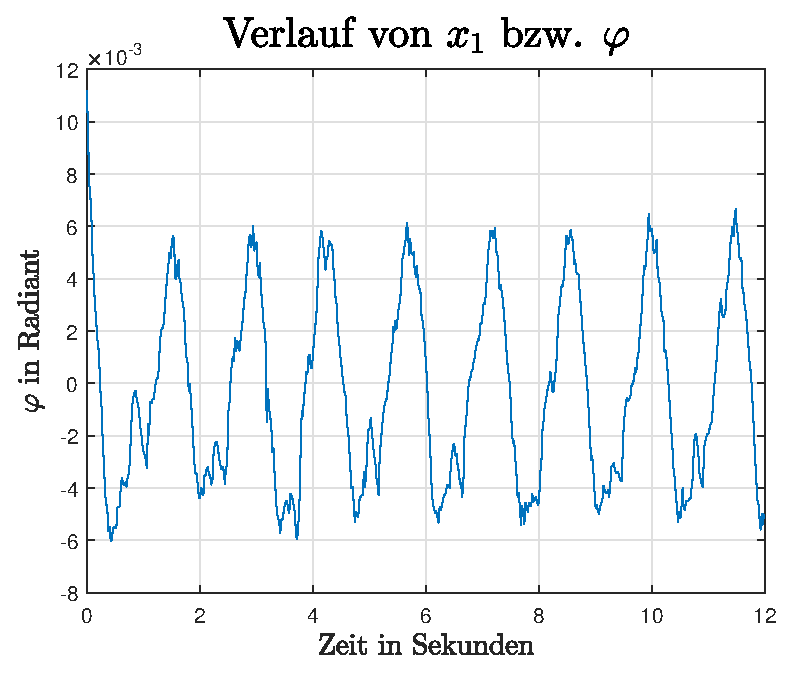
\includegraphics[width=0.45\linewidth]{img/edge_exp3_phi.eps}
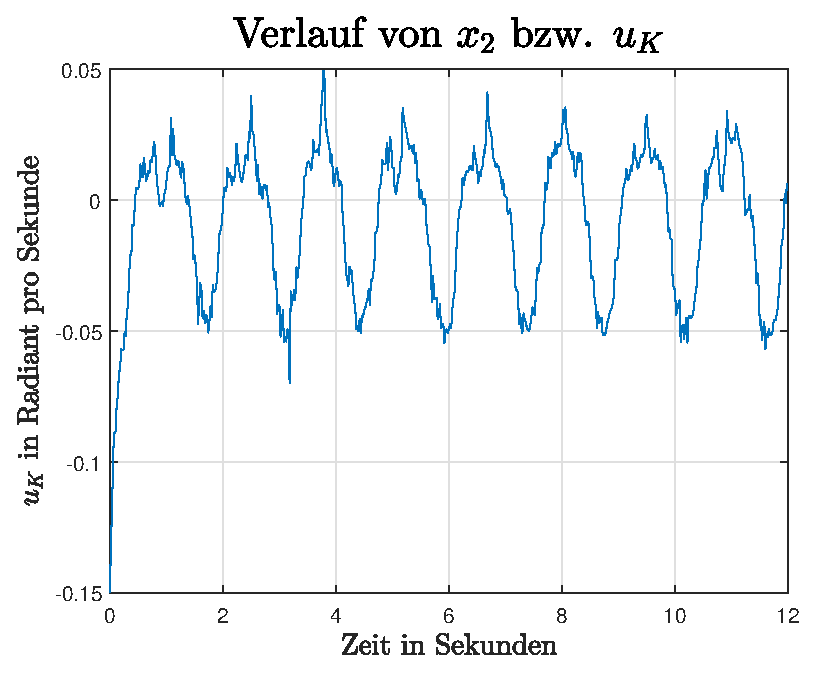
\includegraphics[width=0.45\linewidth]{img/edge_exp3_uk.eps}
\vspace{0.5cm}

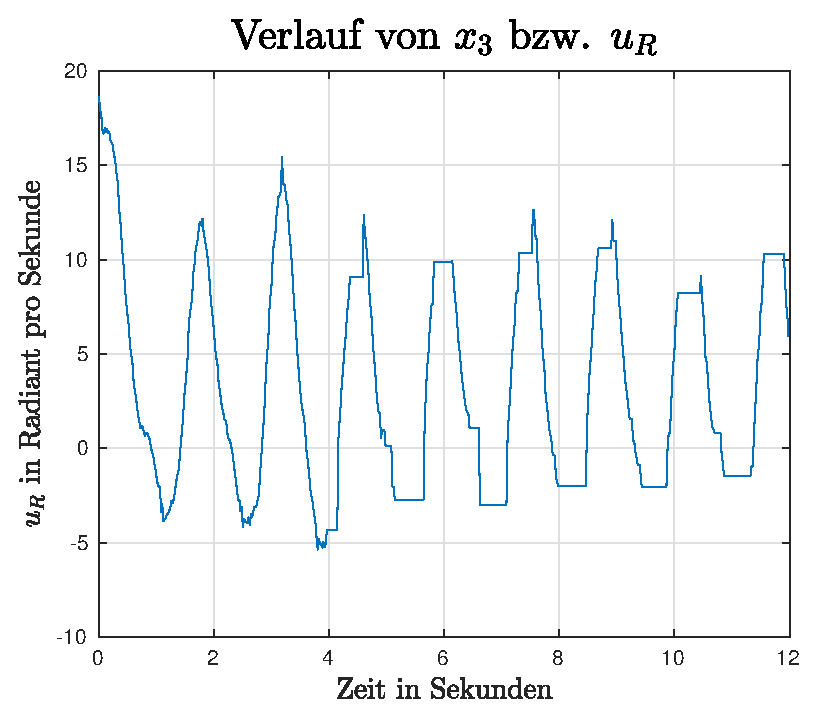
\includegraphics[width=0.45\linewidth]{img/edge_exp3_ur.eps}
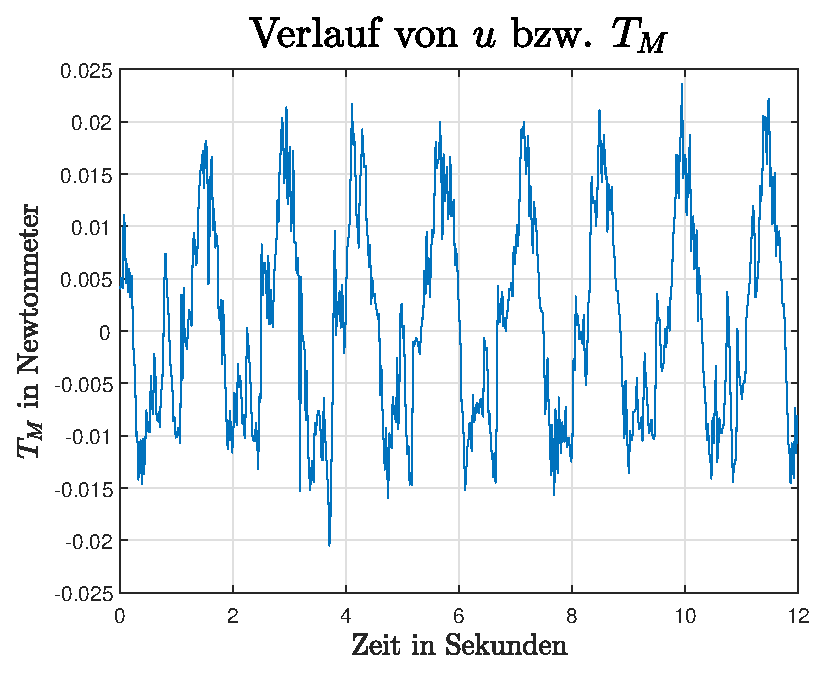
\includegraphics[width=0.45\linewidth]{img/edge_exp3_tm.eps}
\label{plots_phiobs}
\caption{Verlauf des geschätzten Zustandvektors und der Stellgröße, Quelle: eigene Darstellung}
\end{figure}

Der Versuch zeigt, dass das System mit dem Beobachter lediglich grenzstabil ist und mit einer konstanten Amplitude oszilliert. Eine mögliche Begründung für dieses Verhalten ist die Wahl der Beobachtermatrix. Um den Einfluss des Messrauschens zu minimieren wurde die Gewichtungsmatrix $\bs{Q}$ so gewählt, dass eine Beobachtermatrix mit relativ kleinen Elementen resultiert. Hieraus folgt, dass die Eigenwerte des Beobachters nahe an dem Einheitskreis liegen und somit bereits kleine Ungenauigkeiten in den Modellparametern genügen um grenzstabile Eigenwerte zu erhalten. Werden die Eigenwerte des Beobachters näher zu dem Urpsrung gerückt wird der Beobachter allerdings instabil, da das Messrauschen den Schätzwert $\bs{\hat{x}}$ zu stark beeinflusst. Dieses Problem ist darauf zurückzuführen, dass der Luenberger-Beobachter für ein deterministisches System entworfen wird und die stochastischen Störung lediglich indirekt bei dem Entwurfsverfahren berücksichtigt werden. Eine Lösung für dieses Problem stellt das Kalman-Filter dar, welches für die Beobachtung von linearen, zeitvarianten und stochastisch gestörten Systemen genutzt werden kann. Des weiteren bestehen Erweiterung wie das Extended-Kalman-Filter um das Konzept auf nichtlineare Systeme zu übertragen. 
Die Vorteile dieses Ansatz bestehen einerseits darin, dass mit einer Erweiterung auf nichtlineare Systeme ein global gültiges Schätzverfahren entsteht. Andererseits wird durch die Schätzung der Winkel $\varphi_i$ die Anzahl der benötigten Sensoren reduziert. Ebenso kann ein Kalman-Filter genutzt werden um die verrauschten Beschleunigungsmessungen mit den Winkelgeschwindigkeiten zu fusionieren. Im ersten Schritt ist allerdings eine Systemidentifikation und Parameterschätzverfahren durchzuführen, da eine mögliche Ursache für die verbleibende Schwingungen eine geringe Modellgüte ist. Derartige Fehler wirken sich ebenso negativ auf ein Kalman-Filter aus.


\ifx\FORMAT\undefined
\end{document}
\fi
